\documentclass[11pt]{article}

\usepackage[utf8]{inputenc}
\usepackage[T1]{fontenc}
\usepackage{lmodern}
\usepackage[margin=1in]{geometry}
\usepackage{amsmath,amssymb}
\usepackage{booktabs}
\usepackage{graphicx}
\usepackage{caption}
\usepackage{microtype}
\usepackage[round]{natbib}
\usepackage[colorlinks=true,linkcolor=black,citecolor=black,urlcolor=blue]{hyperref}

\bibliographystyle{abbrvnat}

\newcommand{\qtrue}{q(\text{truth})}

\title{\textbf{One Currency, Two Channels:\\
Precision Collapse and the Conditions for Paradigm\\ Lock-In in Multi-Agent Active Inference}}

\author{Mahault Albarracin\\
\small AE Studio\\
\small \texttt{working draft, June 2026}}

\date{}

\begin{document}
\maketitle

\begin{abstract}
Scientific communities sometimes hold an outdated paradigm long after the
evidence against it has arrived. I model this as the collapse of effective
precision on disconfirming evidence, and I ask which mechanisms can produce
that collapse in a population of active-inference agents who share a world.
Three candidate mechanisms are studied on a common substrate: conviction that
attenuates an agent's own observations, material resource limits that price
informative experiments out of reach, and learned trust that reweights
neighbours' reports. The mechanisms turn out to act on a single quantity, the
precision that gates belief updating, but they do not act on the same channel.
Conviction and resources both close the agent's \emph{world} channel, its own
observations, while trust governs the \emph{social} channel, what it hears from
others. The empirical result is that lock-in needs both channels closed at
once. Trust on its own does not lock a community in. It reallocates precision
across sources by predictive accuracy, so it pulls a misled minority toward the
truth whenever some agents can still track the world, and it amplifies error
only once the world channel has already been starved. This makes the
interaction between trust and resources change sign with regime: the two
channels are sub-additive while a reliable signal survives, and super-additive
once it is gone. I locate the boundary as a function of how many truth-tracking
agents remain, and I show that the material channel reproduces textbook
hysteresis, the signature of path dependence familiar from the economics of
increasing returns. The account connects to, rather than competes with, a
companion structural model of paradigm dynamics: that model develops the
conviction channel in depth, and the two channels studied here sit beside it as
the social and material routes to the same precision collapse.
\end{abstract}

\section{Introduction}

A community can have the data and still not change its mind. Priestley measured
the products of combustion as carefully as anyone and kept his commitment to
phlogiston until he died. The pattern is familiar enough that Kuhn made it
central: a paradigm shapes what counts as an anomaly, and a community embedded
in one can absorb a great deal of disconfirming evidence before it
reorganizes \citep{kuhn1962Structure}. The question I want to make precise is
mechanical. Evidence arrives, and it fails to move belief. What, in the
machinery of belief updating, has to be true for that to happen?

Active inference gives a sharp way to ask it. In the free-energy formulation,
the prediction errors that drive belief updating are precision-weighted: a
precision parameter sets the gain on each evidence channel, so high precision
amplifies a surprising observation and low precision attenuates it
\citep{feldmanFriston2010Attention,parrFriston2019Attention}. Belief that does
not move in the face of evidence is, in this language, belief whose evidence
channel has had its precision driven toward zero. I take this as the definition
of lock-in and ask which social, material, and epistemic mechanisms can drive
the precision down.

The dominant formal models of scientific communities do not pose the question
this way. Network epistemology represents each scientist as a scalar credence
in $[0,1]$ over a fixed menu of hypotheses, updated by Bayes and shared across
a communication graph \citep{zollman2010TransientDiversity,
oconnorWeatherall2019Misinformation}. The tradition has real results, Zollman's
among them: a sparsely connected community can outperform a dense one because
slow information flow preserves the diversity that keeps everyone from
converging too early. What a scalar credence cannot carry is the idea that the
gain on the evidence itself is a variable, set by the agent's convictions, its
budget, and whom it trusts. That gain is the object of this paper.

Active-inference accounts of epistemic communities supply one piece of the
answer already. Agents that sample evidence to justify their existing view
accumulate certainty, and past a point that certainty makes them very hard to
move \citep{albarracin2022EpistemicCommunities}. The variational cost of
changing one's mind has been formalized at the single-agent level as a trade
between the informational cost of revision and the utility of the belief held
\citep{hylandAlbarracin2025MindChange}. Both leave room for the question of
what happens when many such agents share a world and reweight each other's
reports, which is where precision stops being a private quantity and becomes a
social one.

This paper makes three claims.

\textbf{Precision is the common currency, and lock-in is a two-channel
condition.} Conviction, material resources, and trust each modulate the
precision on disconfirming evidence, so they are not rival explanations of
lock-in. They split into two channels. Conviction and resources close the world
channel, the agent's own observations. Trust governs the social channel, its
neighbours' reports. A community locks in only when both channels are shut. I
defend this against my own prior expectation that the three would simply
compound (Section~\ref{sec:crosschannel}).

\textbf{Trust corrects more often than it traps, and its interaction with
resources flips sign with regime.} Trust learning reallocates precision across
sources by predictive accuracy, not by headcount, so it follows whoever tracks
the world. It rescues a misled minority whenever accurate agents survive, and
it amplifies error only when material starvation has already removed them. The
trust-by-resource interaction is therefore sub-additive while a reliable
majority survives and super-additive once it does not, and I map the crossing
as a function of the misled fraction (Section~\ref{sec:signflip}).

\textbf{The material channel is path dependence, and it produces hysteresis.}
The cost barrier that gates which experiments an agent can afford is an
increasing-returns switching cost in the sense of Arthur and David
\citep{arthur1994IncreasingReturns,david1985QWERTY}. It produces a hysteresis
loop: a population adapts to a new paradigm, spends down its budget, and then
fails to revert when the truth reverses, even though it sits at the same point
in truth-space it started from (Section~\ref{sec:path}).

The substrates are closed-form and the code is released with the paper.
Everything rests on roughly 250 seeded simulation runs, and where a result is
negative or regime-dependent I report it as such.

\section{Precision as the common currency}
\label{sec:currency}

Fix a community of $N$ agents on a graph. Each agent holds a categorical belief
over a paradigm variable $\theta \in \{1,\dots,K\}$, and the world generates
observations under a fixed true paradigm. An agent updates its belief from two
sources at each step: its own observation of the world, and a trust-weighted
mixture of its neighbours' posteriors. Both updates are precision-weighted, and
the three mechanisms I study each set one of those precisions.

\paragraph{Conviction (epistemic).} An agent whose cherished commitments depend
on the current paradigm down-weights observations that would unseat it. Writing
$\Delta$ for the asymmetry between how much depends on the favoured paradigm and
how much depends on its rival, the weight on the world likelihood takes the form
\[
w \;=\; \exp(-\gamma\,\Delta),
\]
so that as conviction grows the world likelihood is attenuated and the
precision on the agent's own observations falls toward zero. This is the
mechanism developed at length in the companion structural model
(Section~\ref{sec:bridge}); here it is one of three.

\paragraph{Resources (material).} An informative experiment costs more than an
uninformative one, and a depleted agent cannot afford it. The cost of an
experiment $x$ scales with its Fisher information and with how close the agent
is to subsistence,
\[
c \;=\; c_0\,\frac{I_F(x)}{r - r_{\min}},
\]
where $r$ is the agent's resource level and $r_{\min}$ a floor. As $r \to
r_{\min}$ the cost of any discriminating measurement diverges, so the agent is
forced onto low-Fisher, low-precision observations. Resources cap the precision
an agent can buy. This is the active-inference image of bounded, resource-rational
cognition \citep{liederGriffiths2020ResourceRational}.

\paragraph{Trust (social).} Each agent maintains a Gamma-conjugate posterior
over the reliability of each neighbour, updated by the neighbour's predictive
surprisal. Trust does not lower a precision. It \emph{reallocates} precision
across sources, concentrating weight on neighbours who predict well and muting
those who predict badly. Whether that helps depends entirely on who is
predicting well, which is the crux of the results below. Belief sharing of this
kind can sharpen a group's estimate or corrupt it, depending on conditions
\citep{friston2023Federated,catal2024BeliefSharing}.

The two equations and the trust rule make the unifying point concrete. There is
one currency, the precision weighting prediction errors, and there are two
channels it flows through. Conviction and resources both act on the world
channel, the agent's own observations, by different routes to the same
attenuation. Trust acts on the social channel. The rest of the paper is about
what happens when these are switched on together.

\section{Model and substrates}
\label{sec:model}

The experiments use four closed-form substrates that share an inference core. I
describe the core once and then note what each substrate adds. All are pure
categorical Bayes, vectorized over the agent population, with no Monte Carlo.

\paragraph{Inference core.} An agent's generative model is a categorical
likelihood $A$ over observations given a hidden state, a transition $B$, a prior
$D$, and (for policy evaluation only) a preference $C$. State inference is exact
categorical Bayes. The social update replaces the prior at each step with a
trust-weighted mixture of the agent's own carried-forward posterior and its
neighbours' marginal posteriors. Trust weights come from
\verb|build_trust| and \verb|readout_trust_mixture|, shared across substrates.
Graphs come from a Watts--Strogatz, Barab\'asi--Albert, or planted-block
generator \citep{wattsStrogatz1998SmallWorld}.

\paragraph{Hierarchical-context substrate.} The first substrate adds a latent
context variable $c \in \{\text{normal},\text{crisis}\}$ to the state, giving a
joint $(\theta,c)$ carried through a factorized transition $B = B_\theta \otimes
B_c$. Under normal science the paradigm-discriminating columns of $A$ are
averaged, so observations are uninformative about which paradigm is right; under
crisis the discriminating columns are restored. $B_c$ is tridiagonal, with an
anomaly-detection rate that moves an agent toward crisis and a resolution rate
that returns it to normal science. Theory-ladenness is structural here: a
committed agent that reads its data as normal science sees nothing that
discriminates paradigms, which reinforces the normal-science reading, which is a
self-insulating loop. This substrate is the cleanest demonstration that lock-in
can be a property of the dynamics rather than of any single parameter.

\paragraph{Tempered (continuous-$\lambda$) substrate.} The second substrate
lifts the single-agent tempered Bayesian update of
\citet{hylandAlbarracin2025MindChange} to the population. A temperature
$\lambda$ interpolates between full revision and no revision, which lets the
social blend and the revision cost be studied as continuous dials rather than
switches.

\paragraph{Motivated-update substrate.} The third substrate implements the
cost of mind-change as a gate on disconfirming movement rather than as a reward
on the belief state. On the paradigm marginal, the per-step log-update
$\delta(\theta) = \log m_{\text{post}}(\theta) - \log m_{\text{prior}}(\theta)$
is attenuated only when it moves the agent away from a valued paradigm,
\[
w(\theta) = \exp\!\big(-\lambda\,\mathrm{ReLU}(U(\theta))\big), \qquad
\delta_{\text{gated}}(\theta) =
\begin{cases}
\delta(\theta)\,w(\theta) & \delta(\theta) < 0,\\
\delta(\theta) & \delta(\theta) \ge 0.
\end{cases}
\]
Confirming movement flows at full strength and disconfirming movement is
resisted in proportion to utility. The gate is asymmetric and history-dependent,
so it does not saturate to a fixed attractor the way a reward on the state does
(Section~\ref{sec:motivated} returns to why this distinction matters). It is the
flat-substrate version of the conviction channel: utility-driven precision
gating without a dependency network behind it.

\paragraph{Structural substrate.} The fourth substrate carries a per-agent
directed graph of commitments and is the one that hosts all three channels at
once. A propagation operator $T = (I-A)^{-1}$ turns the local dependency matrix
$A$ into total influence. Acting on the unit source it gives a conservatism
field; acting on a utility source it gives the conviction field $U$ that drives
the endogenous $\gamma$ of Section~\ref{sec:currency}. The trust and resource
channels are layered on top. This substrate reproduces the companion model's
conviction mechanism and adds the social and material channels to it, which is
what makes the cross-channel experiments possible.

\section{Experiments}
\label{sec:experiments}

I organize the results around the two-channel claim. Trust alone is studied
first, then trust against resources, then the dose-response and hysteresis of
the material channel, then the full cross-channel factorial that forced me to
revise the thesis, and finally the motivated-update correction. Unless noted,
runs use $K=2$ paradigms with a fixed true paradigm, a heterogeneous prior in
which a minority starts committed to the wrong paradigm, and five seeds per
cell. The readout is the wrong-bloc final belief in the truth, $\qtrue$; low
means locked in.

\subsection{Trust alone accelerates convergence; it does not lock in}
\label{sec:trustalone}

With a clear truth signal and a correct majority (30\% wrong, 70\% right, no
resource limit), turning trust learning on changes the rate of convergence but
not its destination. The asymptotic wrong-bloc belief is identical to three
decimal places with trust off and on (0.993), and the marginal effect of trust
at convergence is on the order of $10^{-4}$. The trajectories differ: without
trust the population reaches 0.99 by about step 70, with trust by about step 20,
a threefold speed-up. The mechanism is that right-bloc agents predict the world
better than wrong-bloc agents, so the Gamma-conjugate update concentrates trust
on them and the misled minority hears a sharper correct signal sooner. Trust is
a predictive-accuracy amplifier. On its own it has no lock-in to contribute,
which already tells us that any lock-in story involving trust has to route
through what happens to that accuracy signal.

\subsection{Trust and resources together: super-additive regression from truth}
\label{sec:trustresource}

The headline interaction appears when trust and resources are both present. On
a $2\times 2$ grid (trust on/off by resources on/off), with the same 30/70 prior
and $c_0=0.12$, the wrong-bloc final beliefs are shown in
Table~\ref{tab:e14}.

\begin{table}[t]
\centering
\caption{Wrong-bloc final $\qtrue$ on the trust-by-resource grid (E14, cont
substrate, $N=30$, 200 steps, 5 seeds). Additivity predicts $0.69$ for the
both-on cell; the observed $0.38$ is a super-additive interaction of $+0.31$.}
\label{tab:e14}
\begin{tabular}{lcc}
\toprule
 & resources off & resources on \\
\midrule
trust off & $0.994 \pm 0.000$ & $0.690 \pm 0.177$ \\
trust on  & $0.994 \pm 0.000$ & $\mathbf{0.381 \pm 0.193}$ \\
\bottomrule
\end{tabular}
\end{table}

Trust alone leaves the wrong bloc fully converged (0.994). Resources alone
partially block it (0.690). If the two contributions were independent the
both-on cell would land near 0.69, and it lands at 0.38. The trajectory in
Figure~\ref{fig:e14} shows what the numbers are doing. With both channels on,
the population rises toward the truth, peaks near 0.80 around step 15, and then
slides back to indecision by step 200. No single-channel condition does this.

The mechanism is the one trust set up in Section~\ref{sec:trustalone}, run in
reverse. As resources drain, agents are gated to low-Fisher experiments and
their observations stop discriminating paradigms. With the world channel
starved, the per-step update is dominated by the social blend. But now no one
predicts the world reliably, so predictive accuracy stops tracking correctness,
and trust concentrates on whoever happens to look accurate in the noise, often
the oscillating wrong-bloc agents. The restoring force toward truth is gone.
Trust without resources amplifies a true signal; trust on top of a starved world
channel amplifies noise.

\begin{figure}[t]
\centering
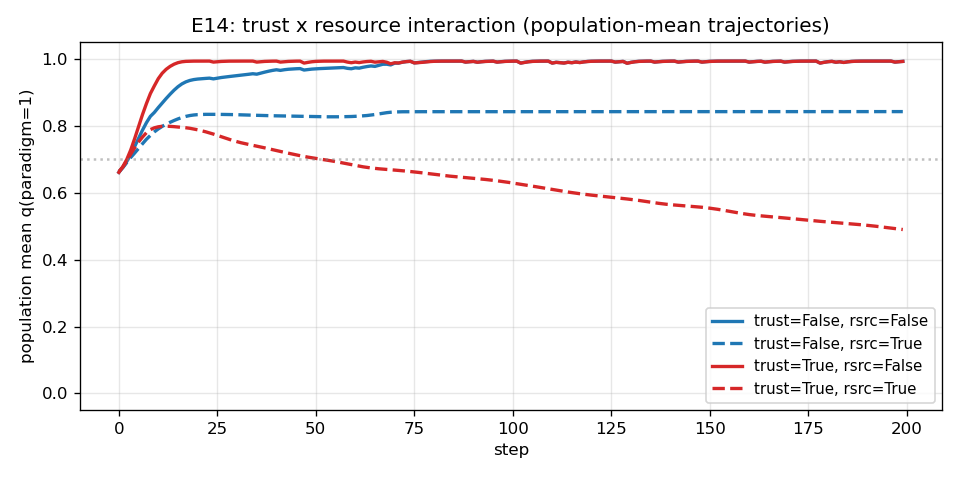
\includegraphics[width=0.8\linewidth]{figures/E14_trajectories.png}
\caption{Wrong-bloc $\qtrue$ over time on the trust-by-resource grid (E14).
The both-on condition (dashed, upper curve at the peak) climbs toward truth,
then regresses to indecision once resources drain. The single-channel
conditions converge or plateau but do not regress.}
\label{fig:e14}
\end{figure}

\subsection{The material channel is a sharp transition}
\label{sec:dose}

Sweeping the cost scale $c_0$ with trust on shows that the resource channel is
not a smooth dial. Between $c_0=0$ and $c_0=0.04$ the population moves from full
adaptation (wrong-bloc 0.99) into the locked regime (wrong-bloc 0.38), and
larger $c_0$ does not lock it in much further (Table~\ref{tab:e15}). Once any
nonzero cost is active, agents drain to the floor $r_{\min}=0.1$ and the system
pins. The correct majority is pulled down with the minority, from 0.99 with no
cost to roughly 0.4 with cost, because drained right-bloc agents lack the
evidential capacity to hold their correct belief against the social signal that
trust amplifies in the starved regime. Resources do not selectively starve the
wrong bloc. They starve everyone, and what separates a converged population from
a locked one is whether agents committed before the budget ran out.

\begin{table}[t]
\centering
\caption{Resource dose-response (E15, cont substrate, trust on, 5 seeds). The
transition is between $c_0=0$ and $c_0=0.04$; there is no smooth gradient.}
\label{tab:e15}
\begin{tabular}{lccccccc}
\toprule
$c_0$ & 0.00 & 0.04 & 0.08 & 0.12 & 0.20 & 0.30 & 0.50 \\
\midrule
wrong-bloc $\qtrue$ & 0.994 & 0.384 & 0.263 & 0.381 & 0.310 & 0.323 & 0.238 \\
final mean $r$ & 1.00 & 0.10 & 0.10 & 0.10 & 0.10 & 0.10 & 0.10 \\
\bottomrule
\end{tabular}
\end{table}

\subsection{Cross-channel: a negative result that fixes the thesis}
\label{sec:crosschannel}

I expected the full factorial to confirm that all three channel pairs compound.
A $2\times2\times2$ design over conviction ($\gamma$), trust, and resources on
the structural substrate, with 30\% of agents committed to the wrong paradigm,
says otherwise (Table~\ref{tab:e18}). All three pairwise interactions are
sub-additive, not super-additive. More striking, the main effect of trust is
\emph{negative}: trust raises wrong-bloc convergence from 0.90 to 0.985, so on
this substrate and regime trust is corrective. Once trust is on, the wrong bloc
converges to truth (about 0.984) almost regardless of $\gamma$ or resources.

\begin{table}[t]
\centering
\caption{Cross-channel cube, wrong-bloc final $\qtrue$ (E18, structural
substrate, $N=30$, 5 seeds). Trust dominates once on; the world-channel
mechanisms ($\gamma$, resources) only bite when trust is off.}
\label{tab:e18}
\begin{tabular}{cccc}
\toprule
$\gamma$ & trust & resources & wrong-bloc $\qtrue$ \\
\midrule
off & off & off & 0.900 \\
off & off & on  & 0.685 \\
off & on  & off & 0.985 \\
off & on  & on  & 0.984 \\
on  & off & off & 0.791 \\
on  & off & on  & 0.685 \\
on  & on  & off & 0.984 \\
on  & on  & on  & 0.984 \\
\bottomrule
\end{tabular}
\end{table}

This contradicts the simple compounding hypothesis, and the mechanism that
explains it is the two-channel picture. A wrong-bloc agent can receive
disconfirming evidence by two routes: from the world, its own observations, and
from society, its neighbours' beliefs. Conviction and resources both close the
world route, conviction by attenuating the world likelihood and resources by
pricing informative experiments out of reach. Neither touches the social route.
In E18 a large correct majority sits on the other end of an open social channel,
so trust rescues the misled bloc and the world-channel mechanisms have nothing
left to bite on. Lock-in needs both channels shut, and E18 only ever shuts one.

This reconciles with E14 rather than contradicting it. E14 starved the world
channel of the whole population, correct agents included, so the social channel
also went dark and trust amplified noise. E18 starved only part of it while a
reliable majority kept predicting, so the social channel stayed informative and
trust used it to correct. The honest statement is that trust's sign is set by
the state of the world channel, which is a sharper claim than uniform
compounding and one the next experiment tests directly.

\subsection{Mapping the sign flip}
\label{sec:signflip}

If the trust-by-resource interaction is sub-additive when a reliable majority
survives and super-additive when it does not, sweeping the size of the misled
bloc should cross the sign. It does. Holding $\gamma$ off to isolate trust and
resources exactly as E14 did, I vary the wrong-bloc fraction and recompute the
$2\times2$ interaction at each (Table~\ref{tab:e19}). The interaction is
sub-additive while a correct majority exists and turns super-additive once the
wrong bloc reaches about 0.8, with the zero crossing between 0.65 and 0.80.

\begin{table}[t]
\centering
\caption{Trust-by-resource interaction vs.\ misled fraction (E19, structural
substrate, $\gamma$ off, 5 seeds). Sub-additive (corrective) until the wrong
bloc dominates, then super-additive.}
\label{tab:e19}
\begin{tabular}{lccccc}
\toprule
wrong fraction & 0.20 & 0.35 & 0.50 & 0.65 & 0.80 \\
\midrule
interaction & $-0.051$ & $-0.137$ & $-0.035$ & $-0.023$ & $+0.070$ \\
sign & sub & sub & sub & sub & \textbf{super} \\
\bottomrule
\end{tabular}
\end{table}

The four-corner view in Figure~\ref{fig:e19} carries a cleaner finding than the
interaction sign alone. Trust-only is the highest curve at every fraction. It
stays corrective even when 80\% of agents are committed to the wrong paradigm,
lifting wrong-bloc belief from 0.045 to 0.296. Trust routes precision by
predictive accuracy, not by how many agents hold a view, and the world generates
the truth, so the agents who predict best are the truth-trackers however few
they are. This is the opposite of follow-the-crowd influence. Trust fails only
when the evidence that makes the truth-trackers accurate is removed, which is
what resource starvation does, and that is the super-additive corner: a small
truth-tracking minority whose accuracy advantage has been starved away. The
magnitude here ($+0.07$) is gentler than E14's cont-substrate $+0.31$, since the
structural substrate has stickier priors and the cost is moderate, but the
direction and the mechanism match.

\begin{figure}[t]
\centering
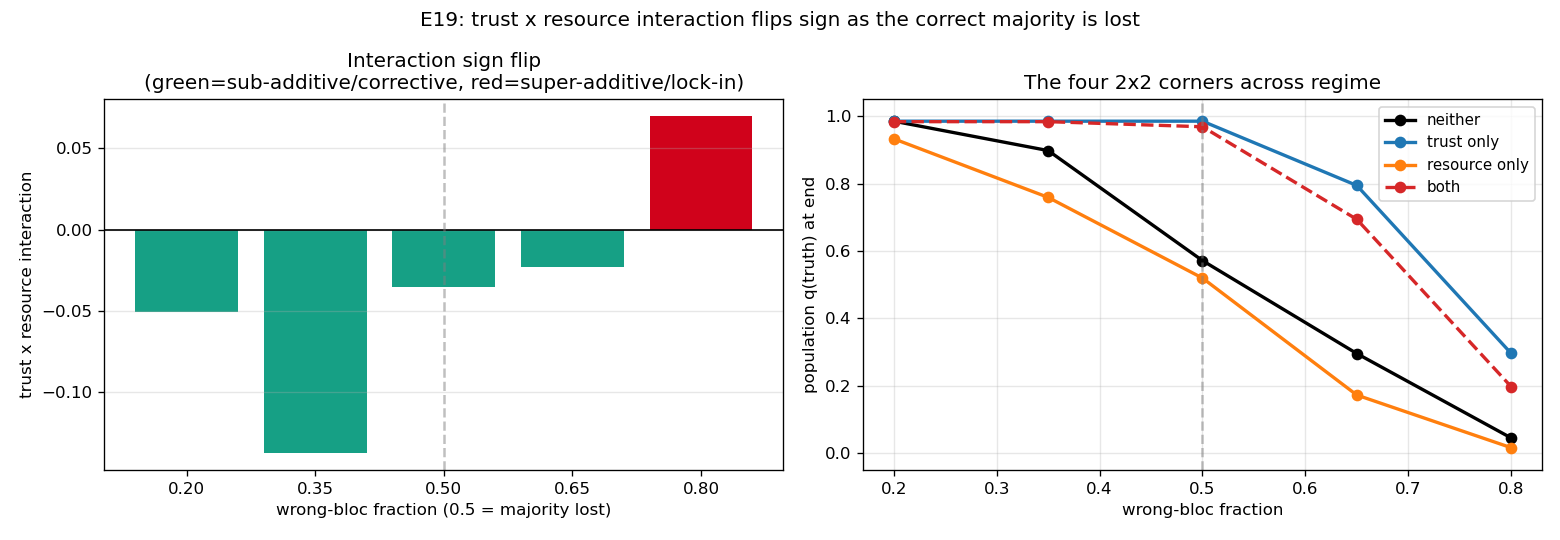
\includegraphics[width=0.95\linewidth]{figures/E19_regime_flip.png}
\caption{Left: the trust-by-resource interaction against the misled fraction,
crossing from sub-additive to super-additive near 0.7. Right: the four
$2\times2$ corners; trust-only (top) is corrective at every fraction.}
\label{fig:e19}
\end{figure}

\subsection{The motivated update, done as a cost of mind-change}
\label{sec:motivated}

An earlier version of the motivated update washed out the social-coupling
boundary: at any positive utility tilt, the population collapsed to a fixed
value across the whole reliability axis. The cause was that the original rule
put a reward on the belief state, $q_\lambda(\theta) \propto q(\theta)
\exp(\lambda U(\theta))$, which acts as a constant external field and pulls the
belief to a fixed point independent of evidence or social context. That is not
what the source theory says. The variational cost of changing one's mind is a
cost on \emph{change}, proportional to the divergence between the new belief and
the prior, not a reward on the state \citep{hylandAlbarracin2025MindChange}.

The corrected rule is the evidence gate of Section~\ref{sec:model}: it resists
disconfirming movement and lets confirming movement flow. With this rule the
social-coupling boundary survives the motivated update. Re-running the original
sweep, the boundary strength (the spread of outcomes across the reliability
axis) holds at 0.75 down to 0.52 as the tilt grows, where the old rule cratered
it to near zero (Figure~\ref{fig:e20}). The diagonal lock-in structure, where
strong social coupling traps the population in the pre-shift paradigm, is
preserved, and a small interpretable interaction appears at high tilt: strong
motivated resistance lets a convicted pro-truth minority cling to its correct
belief against a wrong consensus. Motivated reasoning entrenches whoever an
agent already is, which cuts both ways. As a precision mechanism the gate is the
flat-substrate counterpart of the structural model's endogenous $\gamma$, which
is what lets the motivated substrate join the same two-channel account.

\begin{figure}[t]
\centering
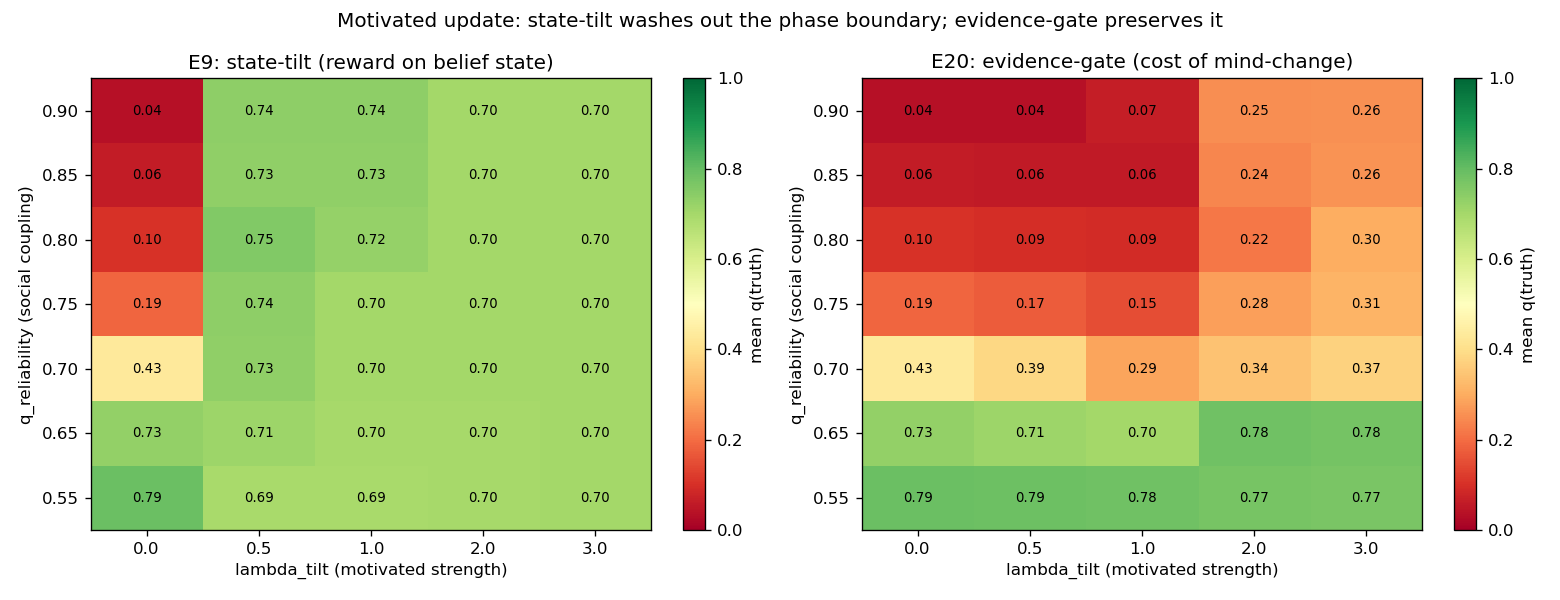
\includegraphics[width=0.95\linewidth]{figures/E20_motivated_gate.png}
\caption{The social-coupling phase boundary under the motivated update. The
reward-on-state rule (left) collapses the boundary for any positive tilt; the
cost-of-mind-change gate (right) preserves it.}
\label{fig:e20}
\end{figure}

\section{Material lock-in as path dependence}
\label{sec:path}

The resource channel has a home in economics. The cost barrier $c =
c_0\,I_F(x)/(r-r_{\min})$ is an increasing-returns switching cost: the more
depleted an agent, the more prohibitive the informative experiment that would
change its mind, so being in a state reinforces staying in it. This is the
positive-feedback mechanism behind Arthur's increasing-returns economics and
David's account of QWERTY, where the technology a market settles on is governed
by the history of adoption rather than by what would be optimal in the abstract
\citep{arthur1994IncreasingReturns,david1985QWERTY}.

The signature of path dependence is hysteresis, and the material channel
produces it. In a two-phase protocol the truth favours a new paradigm in
phase~1 and reverts in phase~2. A population with a slow-biting cost barrier
adapts to the new paradigm in phase~1, spends its budget doing so, and then
cannot afford the experiments that would let it revert in phase~2, even though
phase~2 returns it to the exact truth it started from (Figure~\ref{fig:e16}).
The same point in truth-space supports two different stable population states
depending on the path taken to reach it, which is what path dependence means.
The phase diagram over inflow rate and cost scale (Figure~\ref{fig:e17}) shows
that this is a band rather than a tuned point: there are three regimes, one that
adapts and reverts, one that locks in with hysteresis, and one where adaptation
is blocked from the start, and the hysteresis regime occupies a real region of
parameter space.

\begin{figure}[t]
\centering
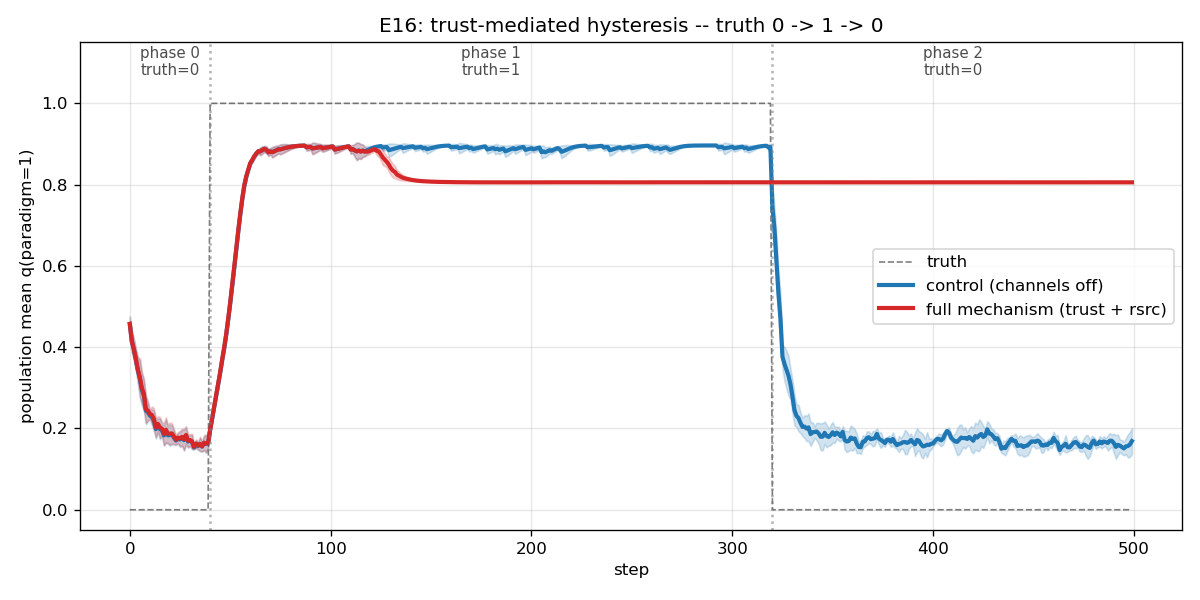
\includegraphics[width=0.8\linewidth]{figures/E16_hysteresis.png}
\caption{Hysteresis under the material channel (E16). The population adapts to
the phase-1 paradigm, drains its budget, and fails to revert when the truth
reverses in phase~2.}
\label{fig:e16}
\end{figure}

\begin{figure}[t]
\centering
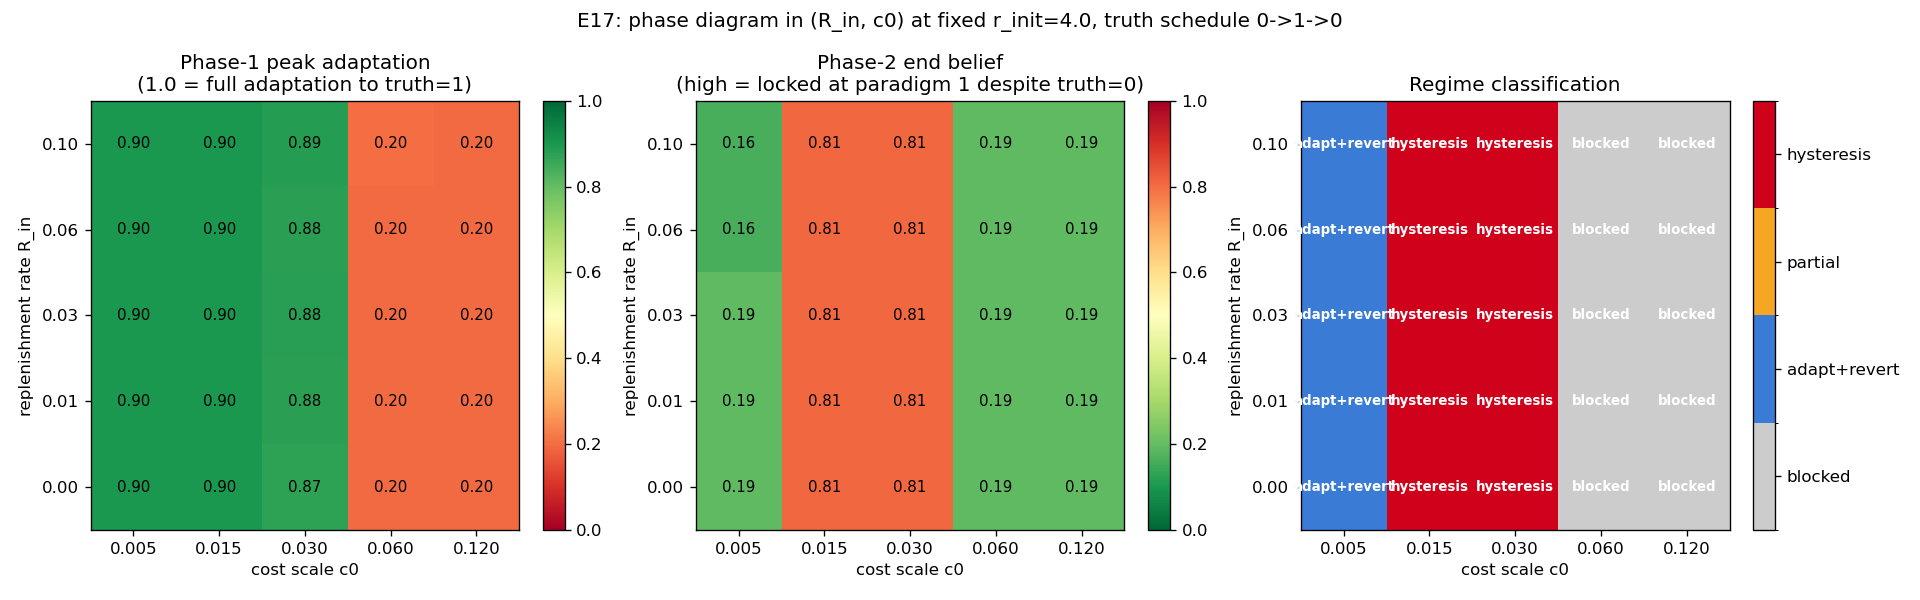
\includegraphics[width=0.8\linewidth]{figures/E17_phase_diagram.png}
\caption{Phase diagram over resource inflow and cost scale (E17): adapt-and-revert,
hysteresis, and blocked regimes. Hysteresis is a band, not a point.}
\label{fig:e17}
\end{figure}

Reading the cost barrier this way gives the model an interdisciplinary handle.
It renders a classical economics-of-science intuition, that a field's history
constrains where it can go, as precision dynamics in a Bayesian community, and
it says when that intuition produces irreversibility.

\section{The bridge to the structural account}
\label{sec:bridge}

A companion manuscript by the same group develops the conviction channel in
full as a structural model of paradigm dynamics: a per-agent Bayesian network of
commitments, the propagation operator $T=(I-A)^{-1}$ that turns local
dependencies into a conviction field, an endogenous $\gamma$ that grows with how
much depends on a paradigm, and structure learning over the dependency graph by
Bayesian model reduction and expansion. That work is the deep treatment of the
epistemic route to precision collapse.

This paper sits beside it on the same currency. The conviction channel here is
the companion model's mechanism, reproduced on the structural substrate so the
connection is shown rather than asserted, and the trust and resource channels
are two routes the companion model does not study. The three modulate the same
precision, and the experiments above show they interact, so the two papers share
a spine rather than competing for the same explanation. The companion model is
the depth on the conviction channel; the contribution here is the unifying
account and the social and material channels, with the conviction channel
carried along as the bridge. The individual-to-collective step that both rely on
is delicate, and the recent work on group-level generative models and on when
belief sharing helps or hurts is the right place to ground it
\citep{heins2024CollectiveBehavior,waade2025AsOneAndMany,friston2024Ecosystems}.

\section{Discussion}
\label{sec:discussion}

The single-currency framing earns its keep by predicting an interaction that
separate-mechanism accounts do not. If trust, resources, and conviction were
independent contributors to lock-in, there would be no reason for the
trust-by-resource interaction to change sign with the size of the misled bloc.
Because all three act on one precision, and because trust acts on a different
channel from the other two, the sign flip follows: trust corrects while the
world channel still carries a signal and amplifies once it is starved. The model
makes the prediction, and the sweep confirms it.

The result also revises a tidy story I went in expecting. Uniform
super-additivity across all three channels would have been cleaner to state, and
it is false. What replaces it is more defensible. Lock-in is a two-channel
condition, and trust is contingent rather than uniformly harmful, which matches
the intuition that a community with even a few reliable members can be pulled
back toward the truth, and that what kills a field is the loss of those members'
ability to demonstrate they are right.

Several limits are worth stating plainly. The magnitude of the sign flip is
substrate- and severity-dependent, $+0.31$ on the tempered substrate and $+0.07$
on the structural one, so I claim the direction and the mechanism, not a
universal number. The full two-dimensional sign-flip surface over misled
fraction and cost scale is not yet mapped; I have the one-dimensional cut. All
runs use $K=2$ paradigms, and higher $K$ may change the social-isolation
dynamics in ways a binary cannot show. The substrates run a Python step loop,
which makes referee-scale robustness sweeps slow, and a scan-and-vectorize
refactor is the prerequisite for finer phase boundaries. None of these touches
the qualitative claims, and each is a concrete next step rather than a caveat
about whether the effect is real.

\section{Related work}
\label{sec:related}

Network epistemology models scientific communities as graphs of Bayesian agents
holding scalar credences, and studies how communication topology shapes
convergence and diversity
\citep{zollman2010TransientDiversity,oconnorWeatherall2019Misinformation}. The
present work keeps the graph and the Bayesian agents and makes the gain on the
evidence the variable of interest, which is what lets paradigm persistence be a
property of precision rather than of topology alone. Active-inference accounts of
epistemic communities supply the precision-based lock-in mechanism this paper
builds on \citep{albarracin2022EpistemicCommunities}, and the variational cost of
mind-change supplies the motivated-update channel
\citep{hylandAlbarracin2025MindChange}. The collective-intelligence literature
on group-level generative models and federated belief sharing gives the
individual-to-collective scaffolding and the warning that aggregation is not free
\citep{friston2023Federated,catal2024BeliefSharing,heins2024CollectiveBehavior,
waade2025AsOneAndMany,friston2024Ecosystems}. The material channel connects to
resource-rational analysis on the cognitive side
\citep{liederGriffiths2020ResourceRational} and to the economics of increasing
returns and path dependence on the social side
\citep{arthur1994IncreasingReturns,david1985QWERTY}. The framing throughout is
Kuhn's \citep{kuhn1962Structure}.

\section{Conclusion}

Paradigm lock-in, in this model, is the collapse of precision on disconfirming
evidence, and it takes two channels to produce. Conviction and material limits
close an agent's window onto the world; trust governs what it hears from others.
A community holds an outdated paradigm when both are shut at once. Trust by
itself does the opposite of locking in, since it follows accuracy and accuracy
follows the world, and it turns harmful only after the world channel has gone
dark. The material channel behaves like an increasing-returns switching cost and
produces hysteresis, so a field can fail to walk back a change it could once
have made. These are three mechanisms and one currency, and reading them that
way predicts how they interact.

\paragraph{Code and data.} The four substrates, experiment configurations, and
seeded results are released with the paper.

\bibliography{refs}

\end{document}
